\section{Reševanje}
\subsection{Podnaloga 1}
Najprej se uverim, da lahko iz začetnih pogojev pravilno integriram časovni razvoj. Izbral sem si nekaj začetnih hitrosti, za katere vemo, kakšne orbite porodijo. Za orbite\footnote{brez upoštevanja simetrije $v_0 \rightarrow - v_0$  in izrojenih elips za $v_0 = 0$} velja:
\[
    \mathrm{orbita}=\begin{cases}
        \mathrm{kro\check{z}nica}, & v_0 = 1,        \\
        \mathrm{hiperbola},        & v_0 = \sqrt{2}, \\
        \mathrm{parabola},         & v_0 > \sqrt{2}, \\
        \mathrm{elipsa},           & \mathrm{sicer}
    \end{cases}
\]

Za \(v_0 \in \left{ 1, \sqrt{2}, 1.5, 0.5, 0.3 \right}\) sem izračunal trajektorije v časovnem intervalu $ t\in\left[ 0, 10\right] $ z adaptivnim časovnim korakom z metodo \texttt{scipy.integrate.solve\_ivp}.

\begin{center}
    \centering
    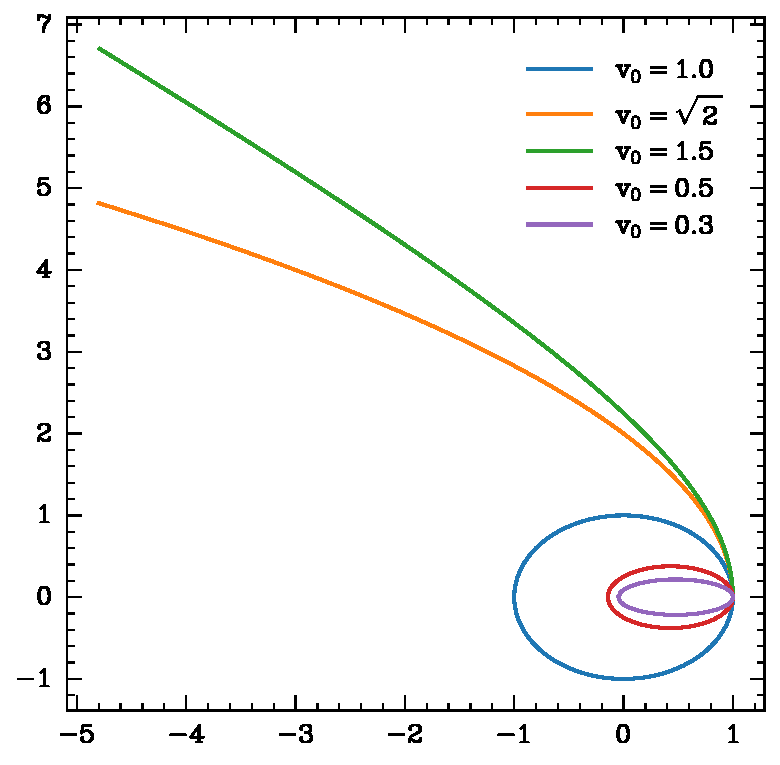
\includegraphics[width=0.5\textwidth]{../images/1-1-v0.pdf}
\end{center}

Naslednji korak je študija invariantnih količin. Zanimalo nas bo spreminjanje polne energije $H$, vrtilne količine $\mathbf{L}$,  in Laplace-Runge-Lenzovega vektorja $\mathbf{A}$ skozi čas za različne začetne pogoje. Rezultate prikazujem na sliki~\ref{fig:1-1-energija}.

\begin{figure}
    \label{fig:1-1-energija}
    \centering
    \begin{subfigure}{0.49\textwidth}
        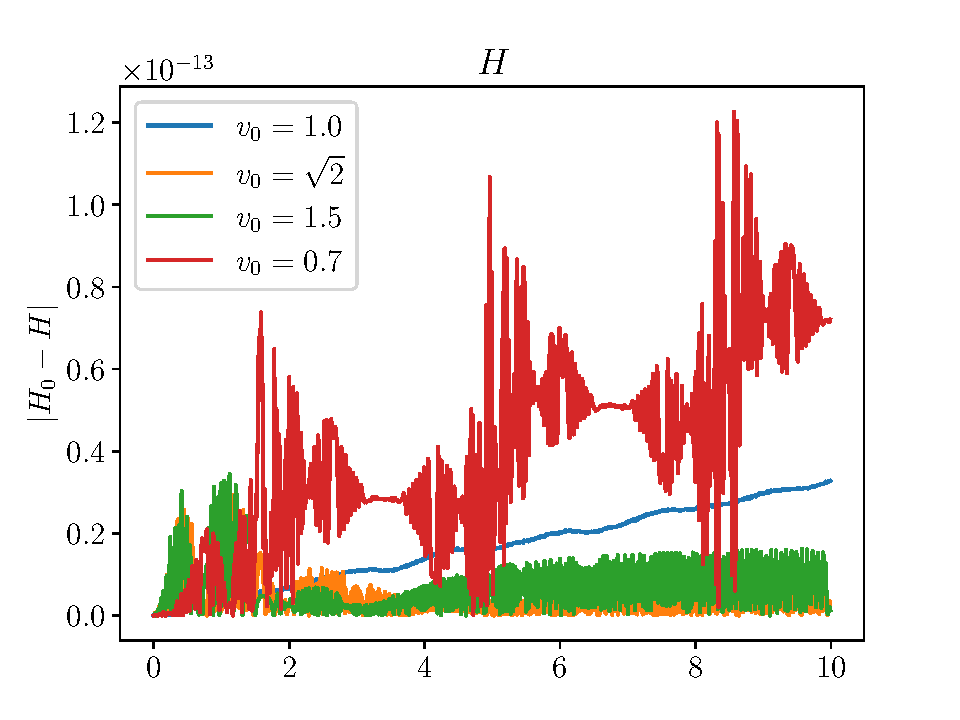
\includegraphics[width=\textwidth]{../images/1-1-H_lin.pdf}
    \end{subfigure}
    \hfill
    \begin{subfigure}{0.49\textwidth}
        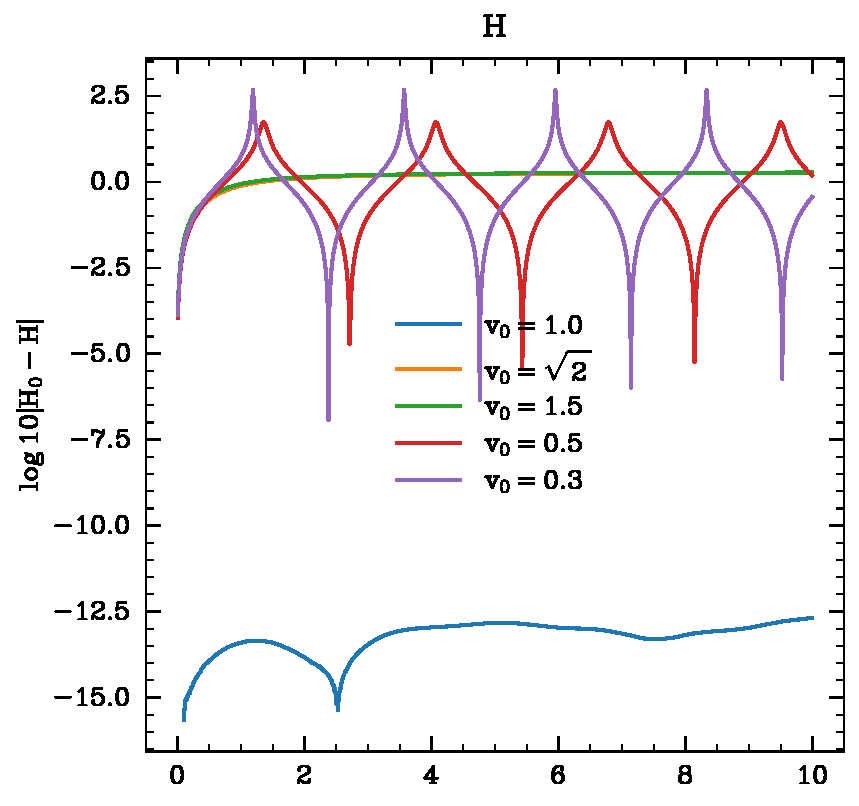
\includegraphics[width=\textwidth]{../images/1-1-H_log.pdf}
    \end{subfigure}
    \newline
    \begin{subfigure}{0.49\textwidth}
        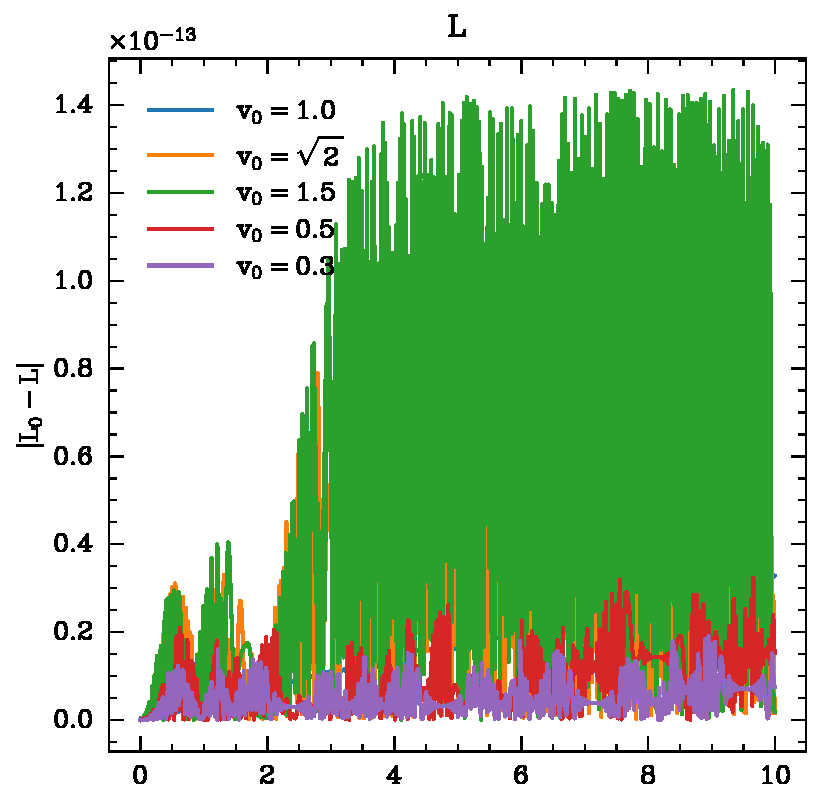
\includegraphics[width=\textwidth]{../images/1-1-L_lin.pdf}
    \end{subfigure}
    \hfill
    \begin{subfigure}{0.49\textwidth}
        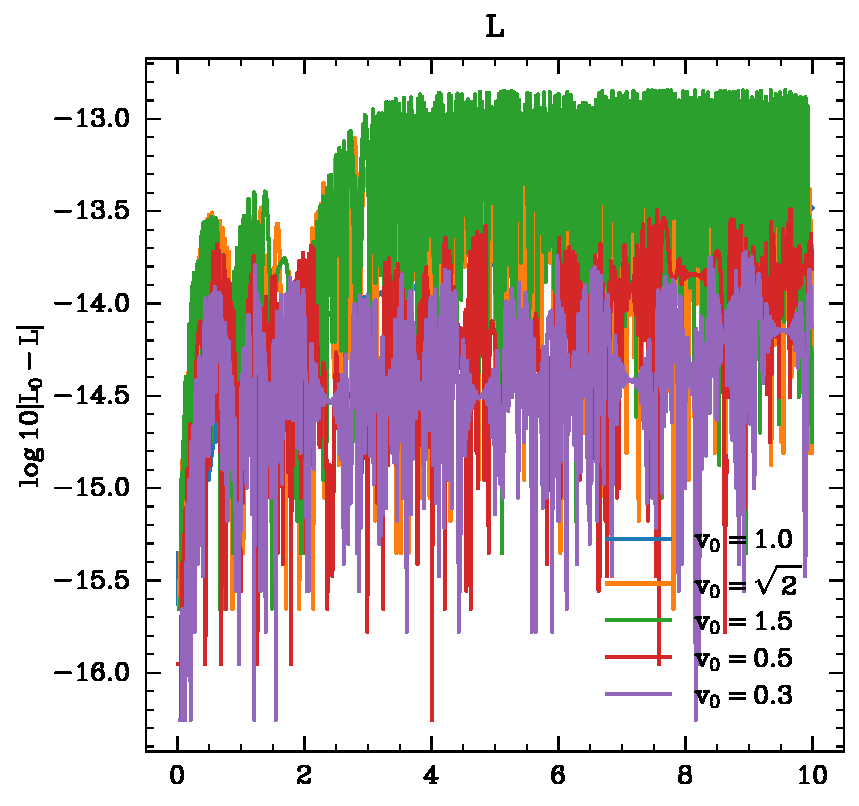
\includegraphics[width=\textwidth]{../images/1-1-L_log.pdf}
    \end{subfigure}
    \newline

    \begin{subfigure}{0.49\textwidth}
        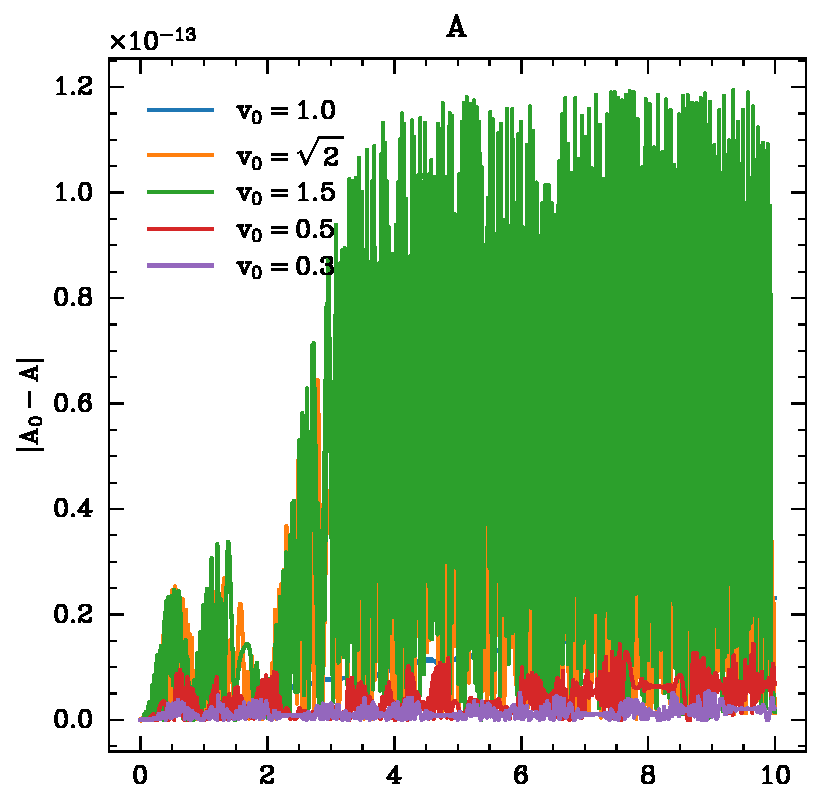
\includegraphics[width=\textwidth]{../images/1-1-A_lin.pdf}
    \end{subfigure}
    \hfill
    \begin{subfigure}{0.49\textwidth}
        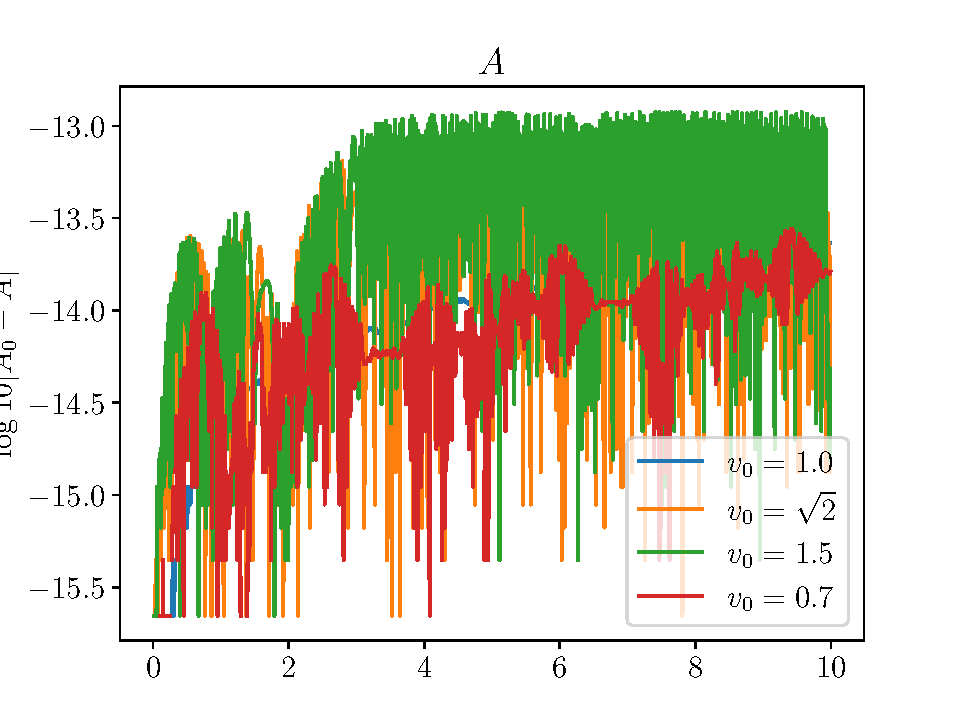
\includegraphics[width=\textwidth]{../images/1-1-A_log.pdf}
    \end{subfigure}
    \caption{Časovni poteki invariantnih količin. V vseh primerih se količine najlepše obnašajo za krožno orbito. Polna energija $H$ je najbolj nestabilna.}

\end{figure}

Za študijo stabilnosti obhodnih časov sem implementiral \texttt{event tracker}, funkcijo, katere koren bo integrator iskal. Pri tem sem se posvetil primerom, ko $v_0<\sqrt{2}$, da zagotovim periodičnost orbit. Uporabljena je bila sledeča metodologija: za vsak $v_0$ sem iskal orbito za $t\in \left(0, 21\pi \right)$, pri čemer mi je prehode čez $y=0$ iskal integrator sam.  Dobljene čase prehoda sem numerično odvajal, da dobim čase med zaporednimi prehodi, nato pa sem izračunal povprečno periodo in standardno deviacijo. Rezultate prikazujem na naslednji sliki.


\begin{center}
    \centering
    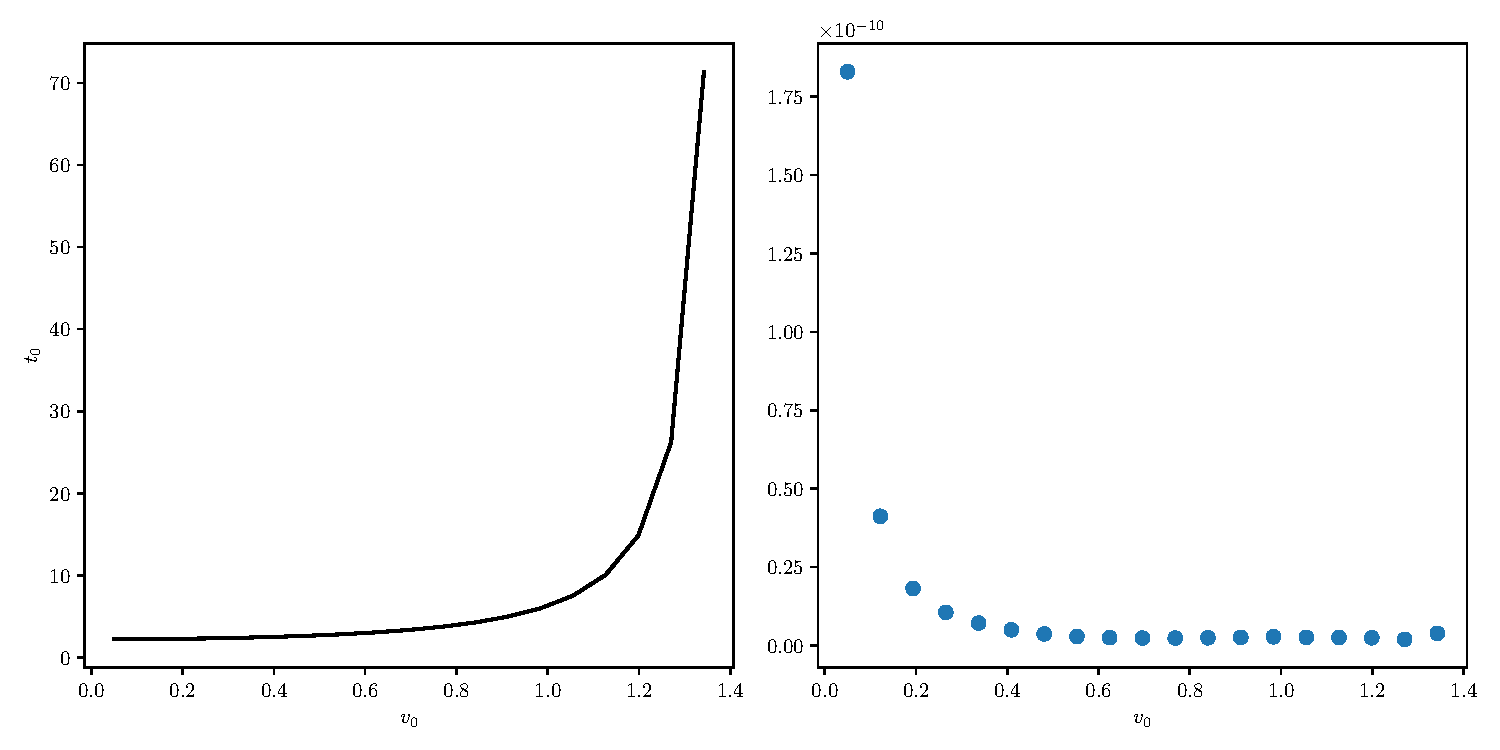
\includegraphics[width=0.9\textwidth]{../images/1-2-t0.pdf}
    {Stabilnost obhodnega časa. [Levo] povprečne vrednosti zaporednih obhodnih časov s standardnimi deviacijami. [Desno] standardne deviacije intervalov med zaporednimi prehodi.}
    % \label{fig:1-2-t0}
\end{center}

Pri nizkih začetnih hitrostih standardna deviacija zaporednih izmerkov strmo naraste, kar lahko pripišemo težavam, na katere naleti integrator v bližini pola potenciala.
\subsection{Podnaloga 2}

Nato sem popravil cevovod za integracijo tako, da je upošteval prispevek dveh pol-sonc, ki krožita okrog skupnega težišča z nastavljivo kotno hitrostjo, nastavljivo medsebojno razdaljo, in nastavljivim zamikom glede na planet.

Raziskal sem, kakšne orbite lahko dobim z različnimi nastavitvami začetnih parametrov. Z rumeno prikazujem orbiti sonc.
\begin{center}
    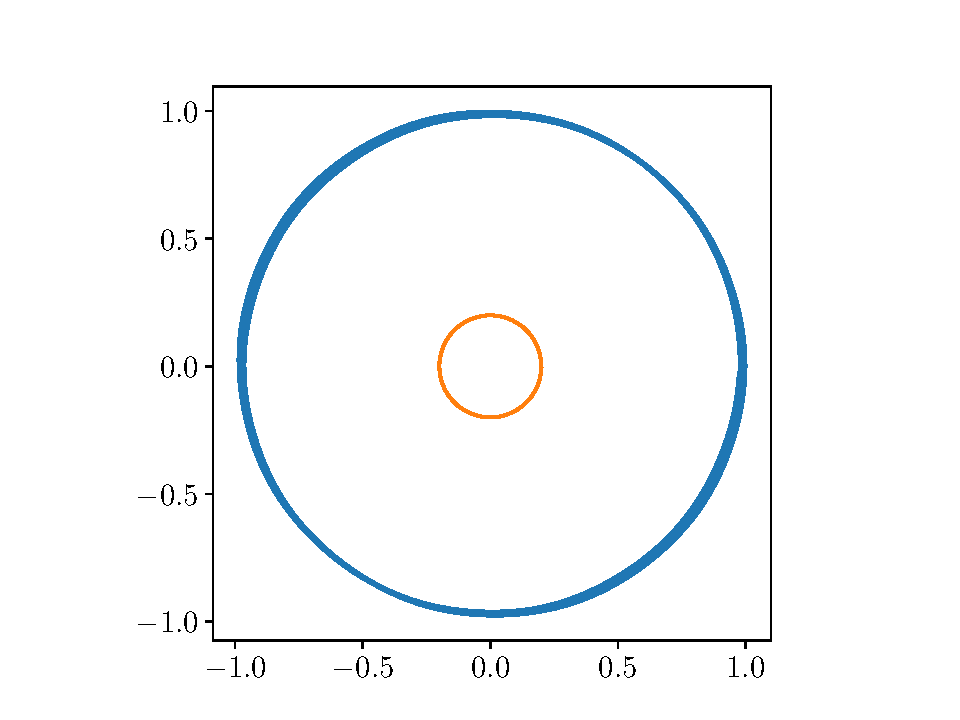
\includegraphics[width=0.5\textwidth]{../images/2-1-orbite_1.pdf}\hfill
    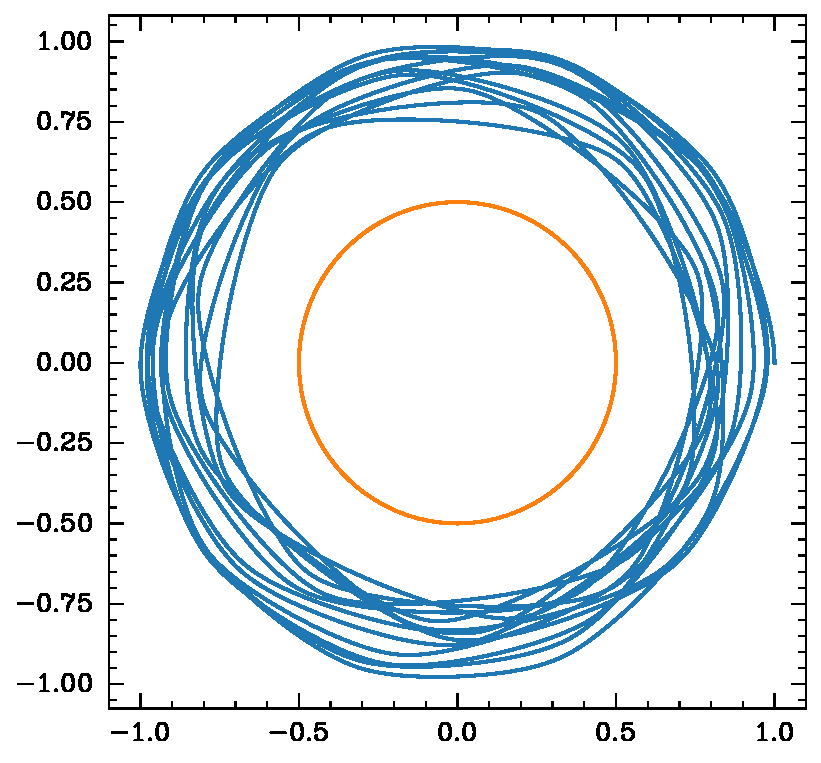
\includegraphics[width=0.5\textwidth]{../images/2-1-orbite_2.pdf}

    % \includegraphics[width=0.5\textwidth]{../images/2-1-orbite_3.pdf}\hfill
    % \includegraphics[width=0.5\textwidth]{../images/2-1-orbite_4.pdf}
\end{center}

Za študijo vpliva dvozvezdja na dinamiko planeta pogledam krožne orbite planeta pri $v_0 = 1$. Z variacijo razdalje med polsoncema~$r$ opazujem, kaj se dogaja s povprečjem in standardno deviacijo oddaljenosti  orbite planeta od masnega središča sistema. V analizo sem vključil samo primere, kjer planet ne 'pobegne'. Kotna hitrost polsonc je v vseh poskusih znašala $2\pi$. Trajektorije sem integriral do časa $t=60$, začetna hitrost planeta je bila fiksirana na $v_0=1$.

Kot pričakovano je vpliv večji pri večjih medzvezdnih razdaljah, ko $r \rightarrow d$, viden pa je že pri majhnih. Presenetljivo je vpliv dvozvezdja bolj opazen, ko je ob času~0 zveznica med polsoncema navpična.

\begin{center}
    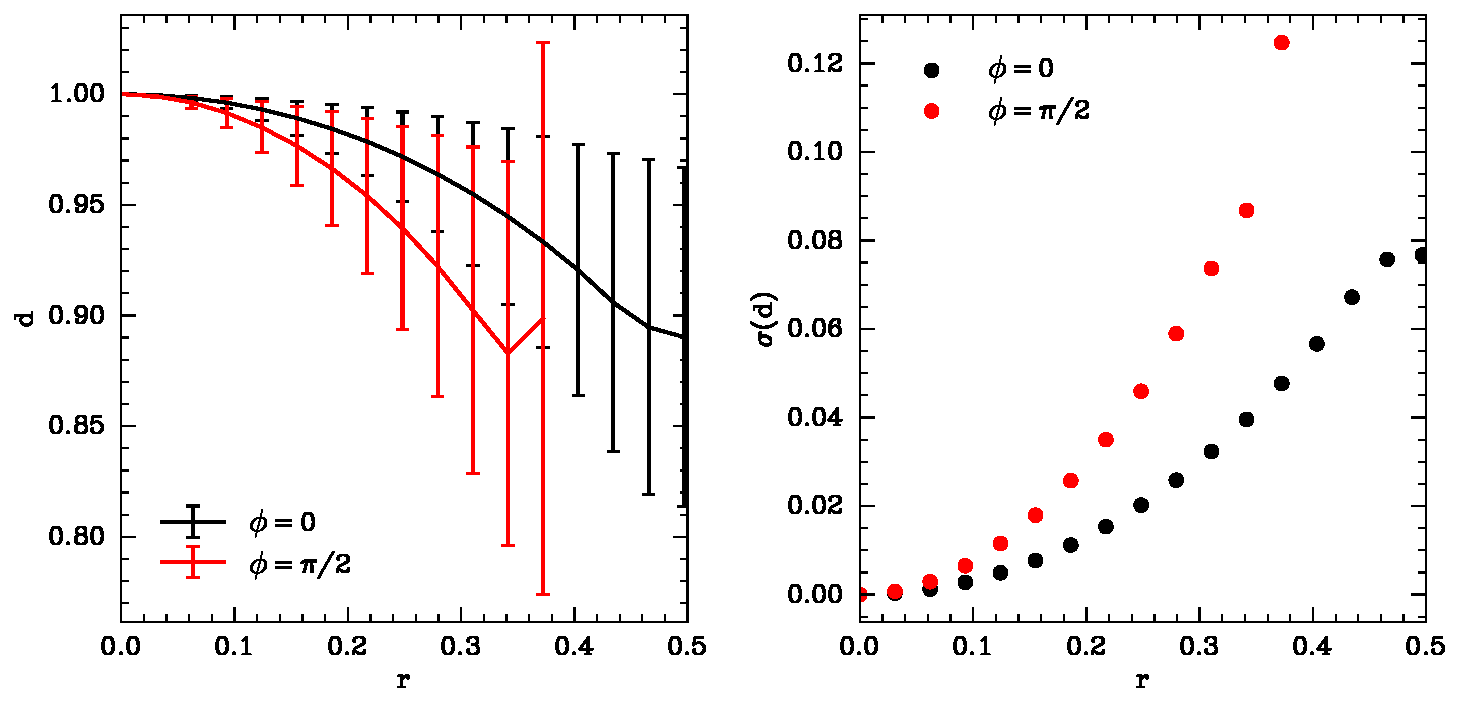
\includegraphics[width=0.9\textwidth]{../images/2-2-vplivr.pdf}
\end{center}
\subsection{Podnaloga 3}

Za študijo preleta mimobežne zvezde sem spet pripravil cevovod za integracijo. Tokrat sem poleg koordinat in impulzov planeta integriral še vodoravno koordinato mimobežne zvezde, kar sem lahko uporabil kot signal za končanje terminacije (kot opisano v prvi podnalogi.) Za začetne pogoje vzamem
\[
    y_0 =
    \begin{bmatrix}
        x \\
        y \\
        v \\
        u \\
        x_2
    \end{bmatrix} =
    \begin{bmatrix}
        \cos{\phi}       \\
        \sin{\phi}       \\
        - v_0 \sin{\phi} \\
        v_0 \cos{\phi}    \\
        -10
    \end{bmatrix},
\]

kjer je $x_2$ vodoravna koordinata mimobežne zvezde. Parametra $\phi$ in $v_0$ si pustim prosta za eksperimentacijo. Za boljši uvid integracijo pustim teči dlje kot naloga zahteva, nato pa po izračunanih trajektorijah izračunam energije $H$, $H_1$, in $H_2$, definirane kot:
\begin{align*}
T &= \frac{u^2 +v^2}{2},\nonumber \\
d_1 &= \sqrt{(x - 0)^2 + (y - 0)^2}\nonumber \\
d_2 &= \sqrt{(x - x_2)^2 + (y - 1.5)^2}\nonumber \\
H &= T - \frac{1}{d_1} - \frac{1}{d_2}\nonumber \\
H_1 &= T - \frac{1}{d_1}\nonumber \\
H_2 &= T - \frac{1}{d_2} \nonumber
\end{align*}

S preletom parametrskega prostora lahko najdem nekaj zanimivih primerov, kjer mimoleteče sonce spremeni orbito planeta, s svojim gravitacijskim privlakom izbije planet iz prvotne orbite, ali pa potegne planet za seboj. Želel sem prečesati prostor parametrov $v_0$ in $\phi$ in s pomočjo značilk $H$, $H_1$, $H_2$ avtomatsko določiti usodo planeta, a na podlagi ročnega opazovanja ne opazim dobre hevristike.

\begin{center}
    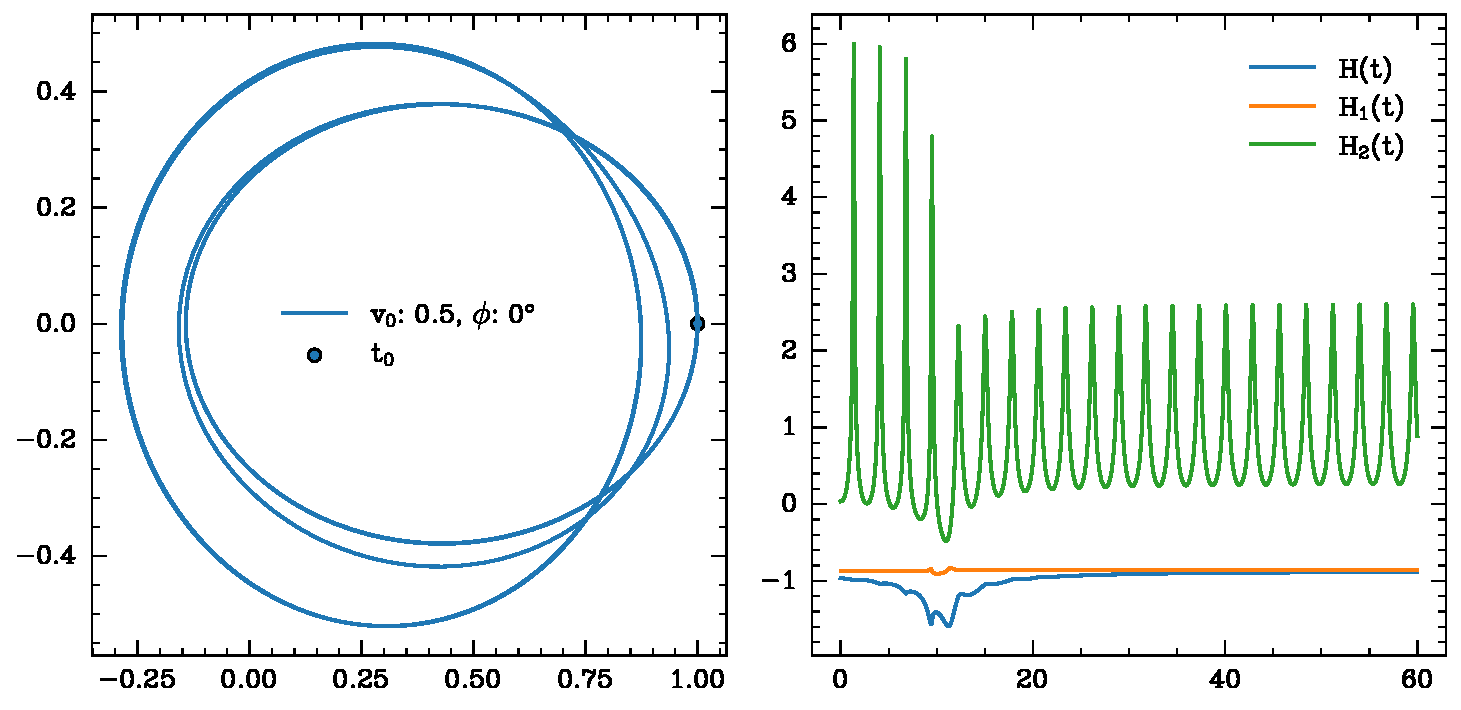
\includegraphics[width=0.9\textwidth]{../images/3-1-0.pdf}
\end{center}
\begin{center}
    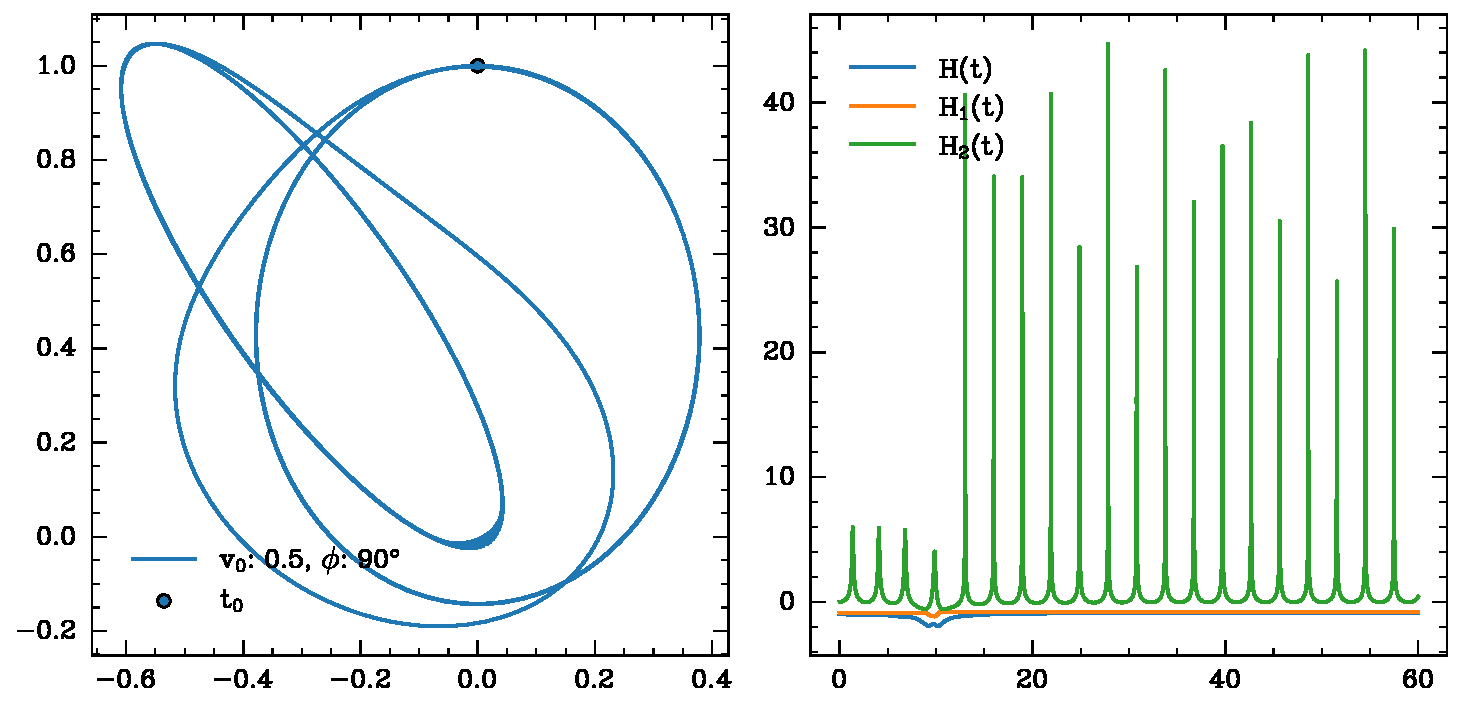
\includegraphics[width=0.9\textwidth]{../images/3-1-2.pdf}
\end{center}

\begin{center}
    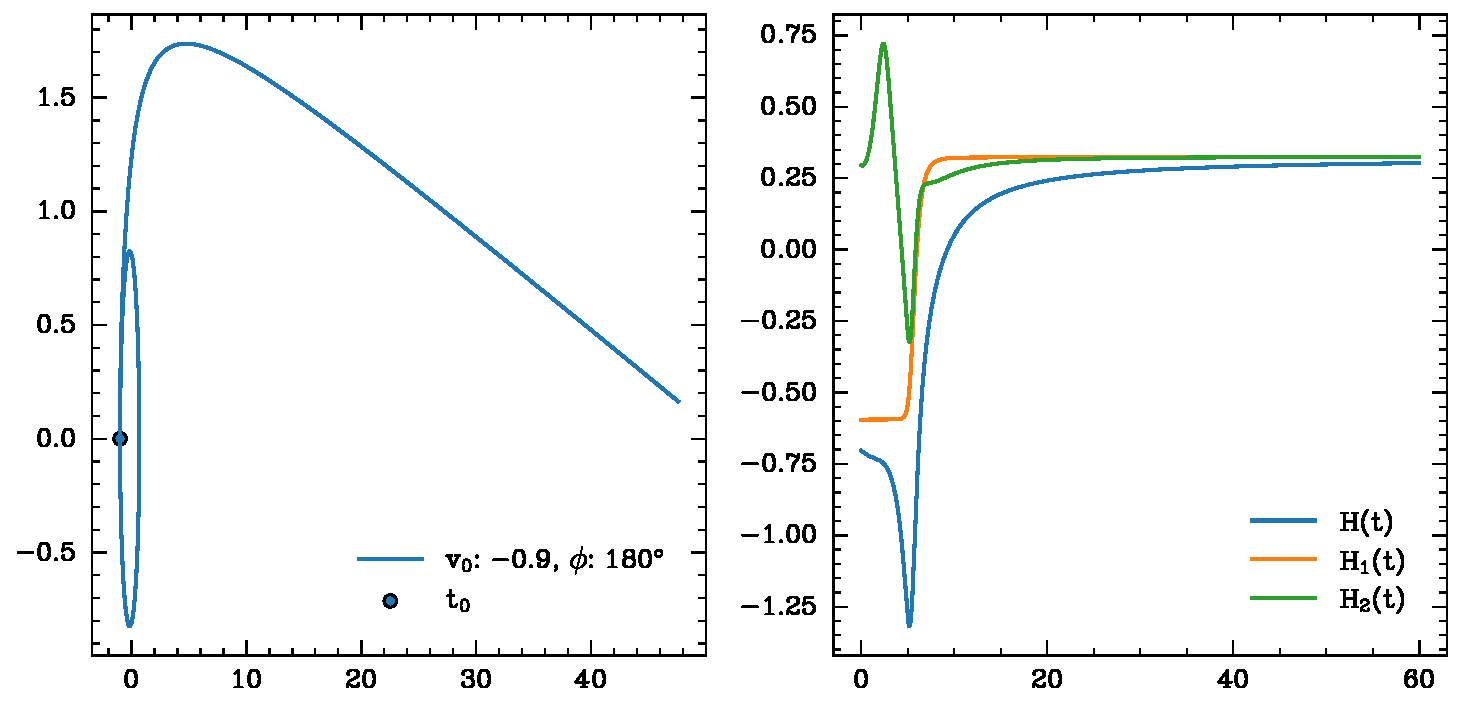
\includegraphics[width=0.9\textwidth]{../images/3-1-60.pdf}
\end{center}
\begin{center}
    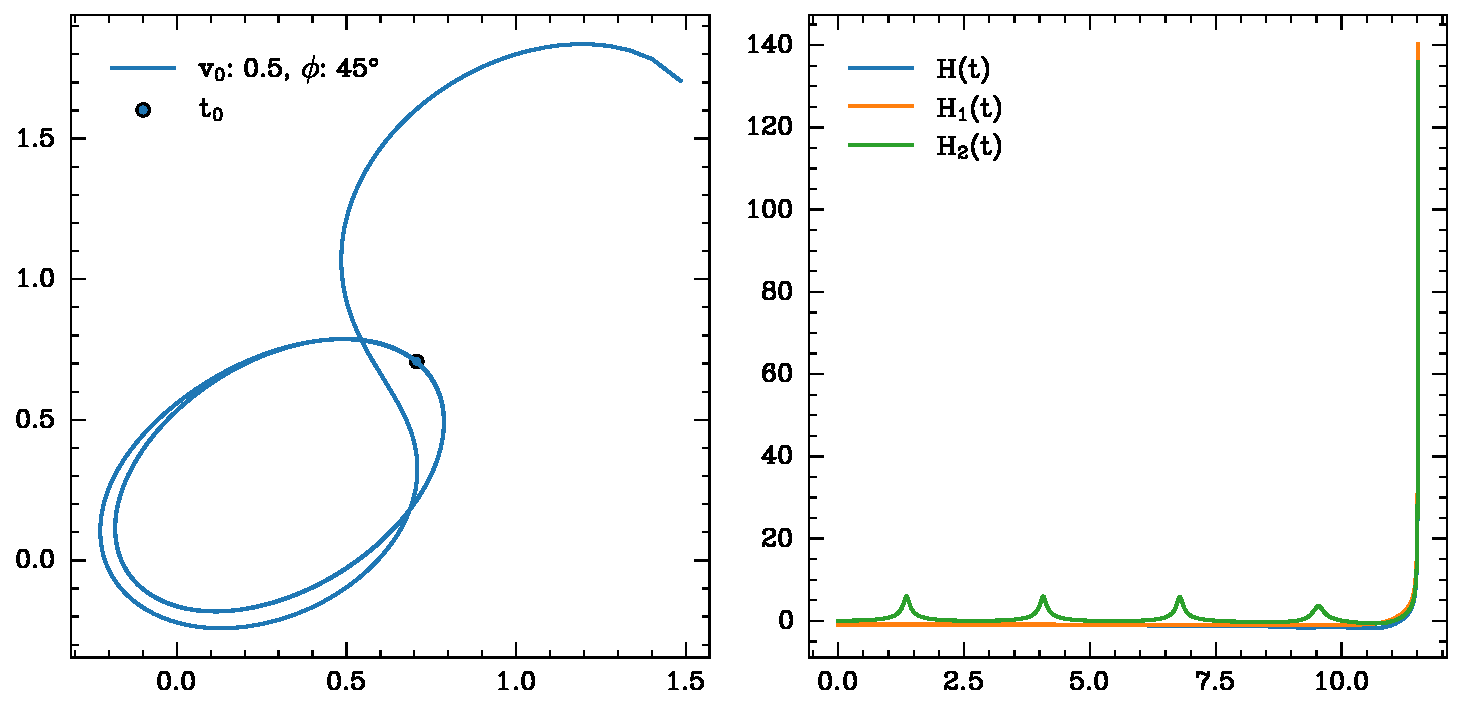
\includegraphics[width=0.9\textwidth]{../images/3-1-1.pdf}
\end{center}
